\section{CFU Implementation}
\label{sec:cfu_impl}

This section describes the two CFU designs developed to accelerate clause
evaluation during inference. In the baseline software implementation, evaluating
a single chunk of a clause requires several instructions to perform the bitwise
masking and comparison. The purpose of the custom instructions is to encapsulate
this work into hardware, reducing instruction count and execution overhead.

Both of the different CFU design are implemented as one or more R4-type instructions using the \texttt{custom-1} opcode. As mentioned Section \ref{sec:neorv32_cfu}, the R4-type format swaps the \textit{funct7} field of the R-type format for an additional source register \textit{rs3}. The three 32-bit source registers are used the store the input word, the positive literal mask and the negative literal mask.

The major difference between the two developed designs is how much of the inference pipeline is moved from software into hardware. The first design offloads only the evaluation of a single chunk, leaving clause voting and class scoring in software. The second design moves the entire scoring pipeline into the CFU, maintaining internal state across instructions so that clause voting and class-score accumulation are performed in hardware.

Both designs operate solely on the operands supplied to them by the CPU and are therefore independent of how the model is stored or loaded. Either design functions correctly with the per-chunk load strategy or the per-class load strategy described in Section~\ref{sec:inference_pipeline}, as the load strategy only determines where the operand words are read from before being passed to the instruction. The benchmark programs used in this work happened to use the per-class strategy, but this choice is incidental to the CFU designs themselves.

The C code snippets shown in this section are abstracted to focus on the CFU instruction calls. References to the model data are shown as a generic \texttt{clause} pointer rather than the specific memory buffer used in the benchmark programs.

\subsection{CFU Design 1: Single-Chunk Processing}
\label{sec:cfu_design1}

The first design implements a single custom instruction that evaluates one 32-bit chunk of a clause. The
operands are defined as follows:

\begin{itemize}
    \item \textit{rs1}: the 32 input bits $X$ for this chunk
    \item \textit{rs2}: the positive mask (PM), where bit $i$ is set if positive
    literal $x_i$ is included in the clause
    \item \textit{rs3}: the negative mask (NM), where bit $i$ is set if negative
    literal $\lnot x_i$ is included in the clause
    \item \textit{rd}: the result, with bit 0 holding the chunk result and bit 1
    holding the all-zero status
\end{itemize}

\subsubsection{Instruction Encoding and Hardware Implementation}
\label{sec:cfu_design1_logic}

The instruction is implemented as a purely combinational circuit, as the
internal logic is simple and the goal is to minimize overhead. It evaluates the
clause-chunk condition shown in Equation~\eqref{eq:chunk_eval} by checking three
conditions in parallel:

\begin{equation}
\text{chunk ok} = \underbrace{((PM \land \lnot X) = 0)}_{\text{positive literals satisfied}}
\;\land\; \underbrace{((NM \land X) = 0)}_{\text{negative literals satisfied}}
\;\land\; \underbrace{((PM \lor NM) \neq 0)}_{\text{chunk not empty}}
\label{eq:chunk_eval}
\end{equation}

The three conditions are explained below:

\begin{enumerate}
    \item Positive literals satisfied: $(PM \land \lnot X) = 0$. If bit $i$ is
    set in PM, then $x_i$ must be 1 in the input. The expression
    $(PM \land \lnot X)$ identifies any included positive literals that are not
    satisfied. If the result is zero, all included positive literals are
    satisfied.

    \item Negative literals satisfied: $(NM \land X) = 0$. If bit $i$ is set in
    NM, then $x_i$ must be 0 in the input. The expression $(NM \land X)$
    identifies any included negative literals that are not satisfied. If the
    result is zero, all included negative literals are satisfied.

    \item Chunk not empty: $(PM \lor NM) \neq 0$. This indicates whether the
    chunk includes any literals at all. A chunk where both masks are zero
    contributes nothing to the clause, and the all-zero status is returned in
    bit 1 so the software can track the all-exclude condition across chunks.
\end{enumerate}

Although the instruction is purely combinational, the NEORV32 CFU introduces a
fixed execution latency. According to the NEORV32 documentation, CFU
instructions incur a minimum overhead of three clock cycles, independent of the
internal logic of the instruction \textcolor{red}{nrv32 datasheet cite}. The full VHDL
implementation is given in \textcolor{red}{fyll ut appendix og ref til det her}.

\subsubsection{Software Integration and Early-Exit Optimization}
\label{sec:cfu_design1_sw}

The instruction is accessed from C through the NEORV32 CFU intrinsic interface,
which translates the call into a single RISC-V instruction. For readability it
is wrapped in a macro, as shown in Listing~\ref{lst:cfu1_macro}.

\begin{code}
\captionof{listing}{Macro wrapping the Design 1 clause-chunk instruction.}
\label{lst:cfu1_macro}
\begin{minted}{c}
#define TM_CFU_CLAUSE_EVAL(x_bits, pos_mask, neg_mask) \
    neorv32_cfu_r4_instr(   \
        TM_FUNCT3_CLAUSE,   \
        (uint32_t)(x_bits), \
        (uint32_t)(pos_mask), \
        (uint32_t)(neg_mask)  \
    )
\end{minted}
\end{code}

For each clause, the software iterates over the 25 chunks, calling the instruction for each non-empty chunk and breaking out of the loop as soon as a chunk fails. The clause output, the all-exclude check, the clause vote, and the class-score accumulation are all handled in software, in the same way as the baseline version. The integration is shown in Listing~\ref{lst:cfu1_c}.

\begin{code}
\captionof{listing}{Software integration of CFU Design 1. The clause vote and 
class scoring are performed in software.}
\label{lst:cfu1_c}
\begin{minted}{c}
for (int j = 0; j < CLAUSES; j++) {
    for (int k = 0; k < POS_CHUNKS; k++) {
        uint32_t pos = clause[k];
        uint32_t neg = clause[POS_CHUNKS + k];

        if ((pos | neg) == 0) continue;
        all_exclude = 0;
        
        // Bitwise checks on positive and negative 
        // literals  is handled in hardware
        uint32_t chunk_ok = TM_CFU_CLAUSE_EVAL(Xi[k], pos, neg);

        if (!chunk_ok) { clause_out = 0; break; }
    }

    clause_out = clause_out && !all_exclude;
    // Score accumulation based on clause polarity
    // (even clauses vote for the class, odd vote against)
    if (clause_out) {
        if ((j & 1) == 0) class_sum++;
        else              class_sum--;
    }
}

\end{minted}
\end{code}

The early exit on the first failing chunk avoids issuing further instructions for a clause that has already failed, mirroring the early-exit optimization used in the baseline software implementation.

\subsection{CFU Design 2: Stateful Clause Processing}
\label{sec:cfu_design2}

The second design moves the full scoring pipeline into the CFU. Rather than returning a per-chunk result for the software to combine, this design maintains internal state across instructions, accumulating clause outcomes into a running class score entirely in hardware. It is implemented as a sequential circuit, with state held in registers between instruction calls.

\subsubsection{Instruction Set and State Management}
\label{sec:cfu_design2_logic}

The design holds three internal state signals: a flag indicating whether the current clause has failed (\texttt{clause\_failed}), a flag indicating whether the current clause has so far included no literals (\texttt{clause\_all\_exclude}), and the accumulated class score (\texttt{class\_score}). Three custom operations, selected by the \texttt{funct3} field, manipulate this state as shown in Figure \ref{fig:cfu_fsm}.

\begin{figure}[H]
    \centering
    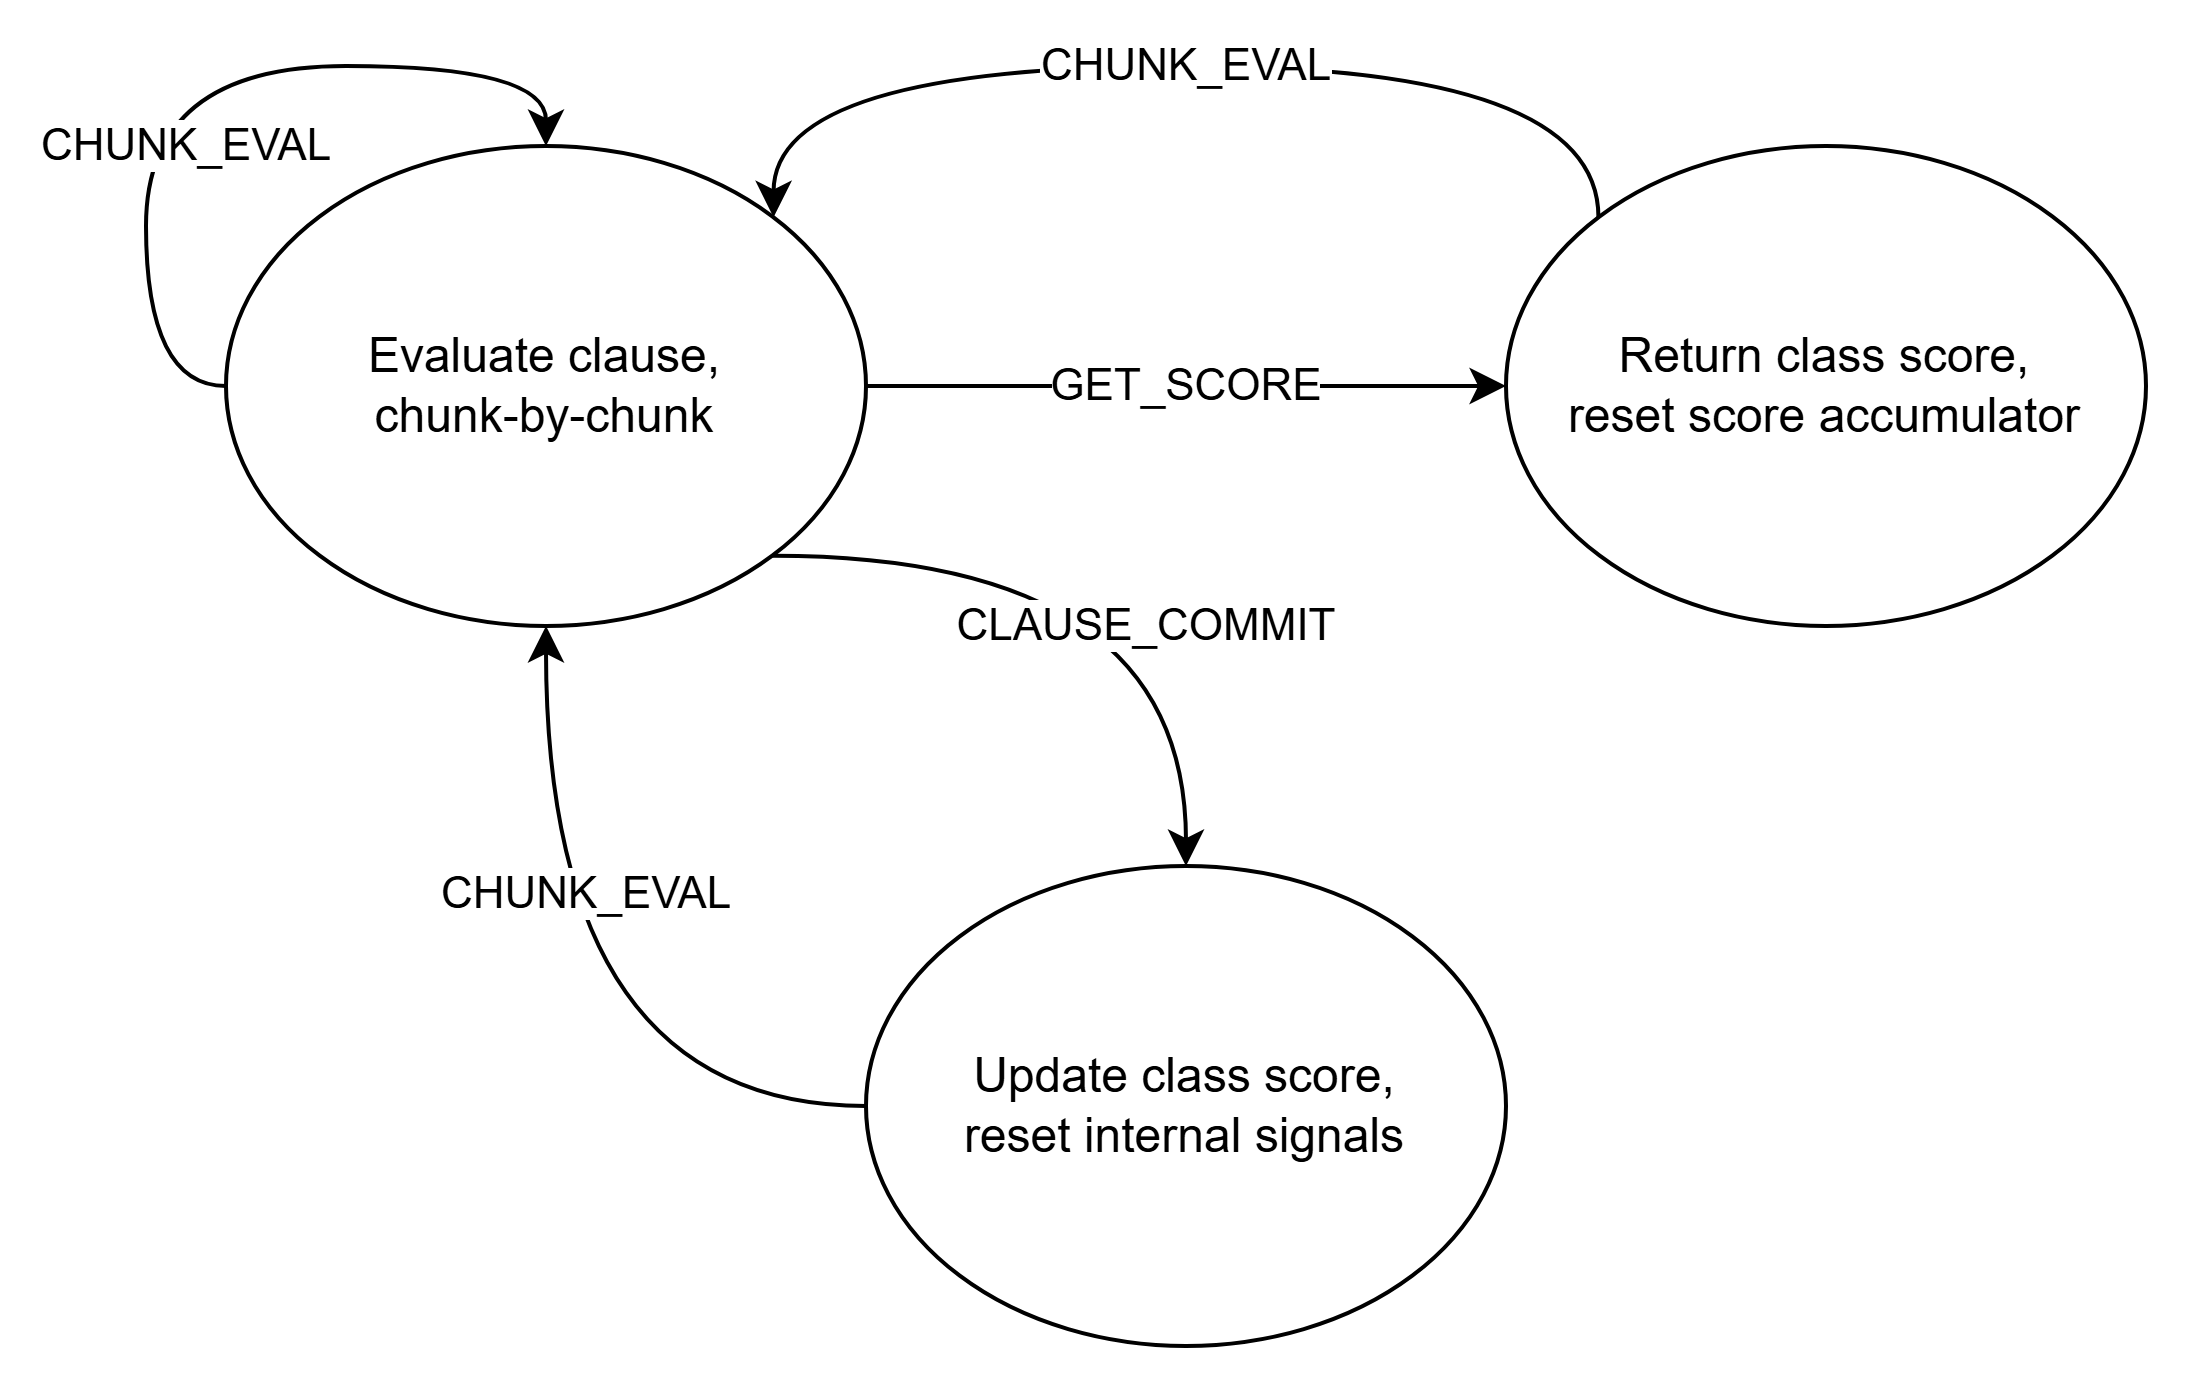
\includegraphics[width=0.9\textwidth]{Figures/cfu2_states.png}
    \caption{State diagram of the second CFU design.}
    \label{fig:cfu_fsm}
\end{figure}

The different instructions implemented in the second design operate as follows:

\begin{itemize}
    \item \texttt{CHUNK\_EVAL} evaluates one chunk using the same mismatch and all-zero logic as in the first design, and updates the clause-failed and all-exclude state accordingly. It returns the current clause-failed status, allowing the software to break out of the chunk loop early once a clause has failed.
    \item \texttt{CLAUSE\_COMMIT} finalizes the current clause. If the clause did not fail and was not all-exclude, it adds the clause vote to the class score, with the vote determined by wether the clause votes for or against the current class, based on the clause id. The clause-failed and all-exclude flags are then reset for the next clause. The class score is clamped to the threshold $T$ during accumulation.
    \item \texttt{GET\_SCORE} returns the final clamped class score as a signed 32-bit value and resets the score accumulator for the next class.
\end{itemize}

By performing the vote accumulation and threshold clamping in hardware, this design removes the per-clause and per-class scoring arithmetic from the software loop entirely. Like in the first design, each operation incurs the fixed three cycle CFU latency, as all operations complete in a single cycle.

\subsubsection{Software Integration}
\label{sec:cfu_design2_sw}

Like in the first CFU design, the different instructions are invoked through C macros, as shown in Listing \ref{lst:cfu2_macros}

\begin{code}
\captionof{listing}{Macros wrapping the three different Design 2 instructions.}
\label{lst:cfu2_macros}
\begin{minted}{c}
#define TM_FUNCT3_CLAUSE_COMMIT 0b001
#define TM_FUNCT3_CHUNK_EVAL    0b000
#define TM_FUNCT3_GET_SCORE     0b010

#define CFU_CHUNK_EVAL(x_bits, pos_mask, neg_mask) \
    neorv32_cfu_r4_instr(          \
        TM_FUNCT3_CHUNK_EVAL,      \
        (uint32_t)(x_bits),        \
        (uint32_t)(pos_mask),      \
        (uint32_t)(neg_mask)       \
    )
#define CFU_CLAUSE_COMMIT(clause_idx) \
    neorv32_cfu_r4_instr(            \
        TM_FUNCT3_CLAUSE_COMMIT,     \
        (uint32_t)(clause_idx),      \
        0,                           \
        0                            \
    )
#define CFU_GET_SCORE() \
    (int32_t)neorv32_cfu_r4_instr( \
        TM_FUNCT3_GET_SCORE,        \
        0,                          \
        0,                          \
        0                           \
    )
\end{minted}
\end{code}


In software, the inner chunk loop calls \texttt{CHUNK\_EVAL} for each non-empty chunk, breaking early if the clause has failed. After the chunk loop, a single \texttt{CLAUSE\_COMMIT} call finalizes the clause. Once all clauses of a class have been processed, a single \texttt{GET\_SCORE} call retrieves the class score. The software no longer tracks clause outputs or accumulates votes, as shown in Listing~\ref{lst:cfu2_c}.

\begin{code}
\captionof{listing}{Software integration of CFU Design 2. Clause voting and class scoring are performed entirely in the CFU.}
\label{lst:cfu2_c}
\begin{minted}{c}
for (int j = 0; j < CLAUSES; j++) {
    const uint32_t *clause = &model[j * WORDS_PER_CLAUSE];

    for (int k = 0; k < POS_CHUNKS; k++) {
        if ((clause[k] | clause[POS_CHUNKS + k]) == 0) continue;

        if (CFU_CHUNK_EVAL(Xi[k], clause[k], clause[POS_CHUNKS + k]) & 1) {
            break;
        }
    }

    CFU_CLAUSE_COMMIT(j);
}

int class_sum = (int)CFU_GET_SCORE();
\end{minted}
\end{code}

\subsection{Design Comparison}
\label{sec:cfu_comparison}

The two designs represent different points on the spectrum of hardware versus
software partitioning of the inference pipeline. Design 1 offloads only the
innermost operation, the evaluation of a single chunk, and leaves all clause
voting and class scoring in software. This keeps the hardware minimal and the
instruction purely combinational. Design 2 offloads the entire scoring pipeline,
performing clause voting, class-score accumulation, and threshold clamping in
hardware, at the cost of a more complex sequential design that must maintain
internal state and that requires additional commit and score-retrieval
instructions per clause and per class.

The motivation for Design 2 was to investigate whether moving a larger portion
of the inference pipeline into hardware would yield a further performance
improvement over Design 1. The performance of both designs relative to the
baseline software implementation is reported and analysed in the next chapter.